\documentclass[../main.tex]{subfiles}

\begin{document}
\begin{problema}
	Considere una cadena de longitud \(L\) y densidad de masa \(\rho\) por
	unidad de longitud. La cadena está apila sobre una mesa fija como
	se muestra en la figura. Determinar la fuerza \(\boldvect\vect{F}\)
	necesaria para levantar la cadena a una velocidad \(\boldvect\vect{\nu}\). Considere
	que hay gravedad.

	\begin{figure}[htb]
		\centering
		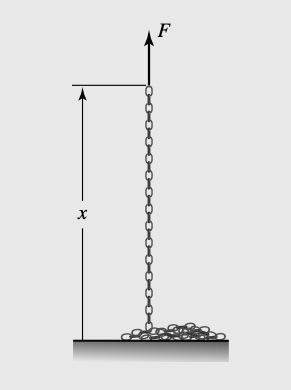
\includegraphics[width=.3\textwidth]{figs/problema01-000.jpg}
	\end{figure}
\end{problema}
\end{document}
